\documentclass[12pt]{article}
\usepackage{amsmath, amssymb, graphicx}
\begin{document}
\title{Chapter 2: Groups \\ Section 5: Equivalence Relations and Partitions}
\author{Alec Mouri}

\maketitle
\section*{Exercises}
\begin{itemize}
\item[(1)]
Denote $\varphi$ to be a map. Consider nonempty fibres $\alpha, \beta$ such that $a \in \alpha \cap \beta$, and: for $x \in \alpha$, $\varphi(x) = X$, and for $y \in \beta$, $\varphi(y) = Y$. So $\varphi(a) = X$, but $\varphi(a) = Y$. Thus, $X = Y$. So, $\alpha = \beta$. Thus, the fibres of $\varphi$ are disjoint.
And, each $x$ is in some fibre of $\varphi$. And by definition each fibre of $\varphi$ is a subset of the domain of $\varphi$. Therefore, the fibres of $\varphi$ form a partition of the domain.
\item[(2)]
Note that $G$ is isomorphic to itself (via the trivial isomorphism). Thus, $G \sim G$.

Suppose $G \sim H$. Then $G$ is isomorphic to $H$, through the isomorphism $\varphi$. Then $\varphi^{-1}$ is also an ismorphism, so then $H$ is isomorphic to $G$, and therefore $H \sim G$.

Suppose $A \sim B$ and $B \sim C$. Then $A$ is isomorphic to $B$ through the isomorphism $\varphi$, and $B$ is isomorphic to $C$ through the isomorphism $\tau$. Then for $a, b \in A$, $\tau(\varphi(ab)) = \tau(\varphi(a)\varphi(b)) = \tau(\varphi(a))\tau(\varphi(b))$. And, $\tau \circ \varphi$ is a bijection, so $\tau \circ \varphi$ is an isomorphism. Thus, $A$ is isomorphic to $C$, and $A \sim C$.
\item[(3)]
Let $A = \left\lbrace a, b, c, d, e \right\rbrace$ be a set of five elements. There are several types of equivalence relations:
\begin{itemize}
\item
There is one partition of 5 elements. There is one such relation.
\item
There is one partition of 4 elements, and one of 1 element. There are 5 such relations.
\item
There is one partition of 3 elements, and one of 2 elements. There are 10 such relations.
\item
There is one partition of 3 elements, and two of 1 element. There are 10 such relations.
\item
There are 2 partitions of 2 elements, and one of 1 element. There are 15 such relations.
\item
There is 1 partition of 2 elements, and three of 1 element. There are 10 such relations.
\item
There are 5 partitions of 1 element. There is 1 such relation.
\end{itemize}
So there are 52 equivalence relations.
\item[(4)]
Let $A = R \cap R'$. Let $a, b, c \in S$. Since $(a, a) \in R, R'$, then $(a, a) \in A$. If $(a, b) \in R, R'$, then $(b, a) \in R, R'$, and so $(a, b) \in A$. If $(a, b), (b, c) \in R, R'$, then $(a, c) \in R, R'$, so $(a, c) \in A$. Thus, $A$ is an equivalence relation.

Let $B = R \cup R'$. Consider $(a, b) \in R$ and $(b, c) \in R'$. But, $(a, c) \not \in R$, and $(a, c) \not \in R'$. So $(a, c) \not \in B$. So $B$ is not an equivalence relation.
\item[(5)]
Let $a, b, c \in H$. Since $a^{-1}a = 1 \in H$, then $a \sim a$. Suppose $a \sim b$. Then $b^{-1}a \in H \rightarrow a^{-1}b \in H$, so $b \sim a$. Suppose $a \sim b$ and $b \sim c$. Then $b^{-1}a \in H$ and $c^{-1}b \in H$, so $c^{-1}bb^{-1}a = c^{-1}a \in H$. So $a \sim c$. Thus, $a \sim b$ is an equivalence relation.
\item[(6)]
\begin{itemize}
\item[(a)]
Let $a, b, c \in G$. Since $1a1^{-1} = a$, then $a \sim a$. Suppose $a \sim b$. Then for some $x$, $xax^{-1} = b \rightarrow a = x^{-1}bx = (x^{-1})^{-1}bx^{-1}$, so $b \sim a$. Suppose $a \sim b$ and $b \sim c$. Then for some $x, y$, $xax^{-1} = b$ and $yby^{-1} = c$. Then $c = yxax^{-1}y^{-1} = yxa(yx)^{-1}$. So $a \sim c$. 
\item[(b)]
If $a$'s conjugacy class consists only of $a$, then for all $b$, $bab^{-1} = a \rightarrow ba = ab$. So, $a$ is a member of the center of $G$.
\end{itemize}
\item[(7)]
According to the reflexive property, $(x, x) \in R$. This corresponds to the line $y = x$.

According to the symmetric property, if $(x, y) \in R$, then $(y, x) \in R$. Note that if $(x, y)$ is reflected across the line $y = x$, then we have $(y, x)$. So, $R$ includes the line $y = x$, and is symmetric about $y = x$.
\item[(8)]
\begin{itemize}
\item[(a)]
Let $a \in \mathbb{R}$. Clearly, $(a, a) \in R$, so $R$ is reflexive. 

Let $(a, b) \in \mathbb{R}$. Then $a = b$. So, $(b, a) \in \mathbb{R}$. So $R$ is symmetric. 

Let $(a, b), (b, c) \in \mathbb{R}$. Then $a = b = c$. So $(a, c \in \mathbb{R}$. So $R$ is transitive. 

Thus $R$ is an equivalence relation.
\item[(b)]
$R$ is not reflexive, since for $x \in \mathbb{R}$, $(x, x) \not \in R$.

$R$ is symmetric, since $(a, b) \not \in R$ for $a, b \in \mathbb{R}$.

$R$ is transitive, since $(a, b) \not \in R$ for $a, b \in \mathbb{R}$.
\item[(c)]
$R$ is not reflexive, since $(1, 1) \not \in R$.

$R$ is not symmetric, since $(1, 0) \in R$, bit $(0, 1) \not \in R$.

Let $(a, b), (b, c) \in R$. Since $b = c = 0$, then $(a, c) = (a, 0) \in R$. So, $R$ is transitive.
\item[(d)]
$R$ is not reflexive, since $(0, 0) \not \in R$.

Suppose $(a, b) \in R$. Then $ab + 1 = 0 \rightarrow ba + 1 = 0$, so $(b, a) \in R$, and $R$ is symmetric.

Let $a = 1, b = -1, c = 1$. Then $ab + 1 = bc + 1 = 0$, so $(a, b), (b, c) \in R$. But $ac + 1 = 2$, so $(a, c) \not \in R$. So $R$ is not transitive.
\item[(e)]
Let $x \in \mathbb{R}$. Then $x^2x - xx^2 - x + x = 0$, so $(x, x) \in R$. So $R$ is reflexive.

Let $(x, y) \in R$. Then $x^2y - xy^2 - x + y = 0 \rightarrow 0 = -(x^2y - xy^2 - x + y) = y^2x - yx^2 - y + x$. Therefore, $(y, x) \in R$, and $R$ is symmetric.

Let $(a, b), (b, c) \in R$. Fixing $b$, we know that $a^2b - ab^2 - a + b = 0$ has two possible solutions for $a$, one of which is $b$. And, $c^2b - bc^2 - b + c = 0$ again has two solutions: in fact they have the same solutions. Suppose $a = b$. Then trivially, $(a, c) = (b, c) \in R$ Similarly, if $c = b$, then $(a, c) = (a, b) \in R$. If $a \neq b$ and $c \neq b$, then $a = c$. So, $(a, c) = (a, a) \in R$ from reflexivity. Thus, $R$ is transitive.

Thus $R$ is an equivalence relation.
\item[(f)]
Let $x \in \mathbb{R}$. Then $x^2 - xx + 2x - 2x = 0$. So $R$ is reflexive.

Let $a = -2, b = 0$. Then $a^2 - ab + 2a - 2b = 4 - 0 - 4 - 0 = 0$ So $(-2, 0) \in R$. But $b^2 - ba + 2b - 2a = 0 - 0 + 0 - 2(-2) = 4 \neq 0$. So $(b, a) \not \in R$. So $R$ is not symmetric.

Let $(a, b), (b, c) \in R$. So $a^2 - ab + 2a - 2b = (a+2)(a - b) = 0$. So, either $a = -2$, or $a = b$. If $a = b$, then $(a, c) = (b, c) \in R$. If $a = -2$, then since $c$ is arbitrary, then $(a, c) \in R$. So $R$ is transitive.
\end{itemize}
\item[(9)]
Suppose $R$ is the set of all points that satisfies $0 = \prod_{i=-\infty}^{\infty}(x - y - i)$

Then, for all $x \in \mathbb{R}$, $(x, x) \in R$, so $R$ is reflexive.

For $(a, b) \in R$, then $0 = \prod_{i=-\infty}^\infty(a - b - i) = \prod_{i=-\infty}^\infty(b - a - i)$, so $(b, a) \in R$. So $R$ is symmetric.

Let $(a, b), (b, c) \in R$. If $a = b$, then $(a, c) \in R$. Similarly, if $b = c$, then $(a, c) \in R$. Suppose $a \neq b$ and $b \neq c$. Let $a - b - j = b - c - k = 0$, for some $k$. Then $a - c - (j + k) = 0$. So, $(a, c) \in R$. So $R$ is transitive.

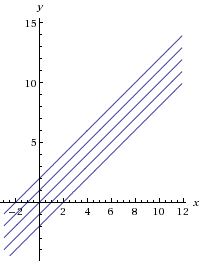
\includegraphics[scale=1]{9}
\item[(10)]
Graph: \\
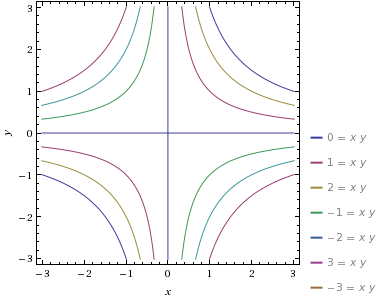
\includegraphics[scale=1]{10}
\item[(11)]
$$\overline{0} + \overline{0} = \overline{1} + \overline{1} = \overline{0}$$
$$\overline{1} + \overline{0} = \overline{1}$$
$$\overline{0}\cdot\overline{0} = \overline{0}\cdot\overline{1} = \overline{0}$$
$$\overline{1}\cdot\overline{1} = \overline{1}$$
Note that the commutative, associative, and distributive properties of addition and multiplication hold as well.
\item[(12)]
Consider the coset $aN$ and the fiber of $\varphi$ on $a$, $\varphi^{-1}(a)$. Consider $g \in \varphi^{-1}(a)$, ie. $g$ is a member of the fiber of $\varphi$ on $a$. Then $\varphi(g) = \varphi(a)$. So $g \in aN$, and $\varphi^{-1}(a) \subseteq aN$. And, if $g \in aN$, then by definition $\varphi(g) = \varphi(a)$, so $g \in \varphi^{-1}(a)$. And $aN \subseteq \varphi^{-1}(a)$. Thus, $aN = \varphi^{-1}(a)$. Therefore the cosets are precisely the fibres of $\varphi$.
\end{itemize}
\end{document}